%%%%%%%%%%%%%%%%%%%%%%%%%%%%%%%%%%%%%%%%%
% Beamer Presentation - Final Defense
% Master's Thesis Final Presentation
%%%%%%%%%%%%%%%%%%%%%%%%%%%%%%%%%%%%%%%%%

\documentclass{beamer}

\mode<presentation> {
\usetheme{Madrid}
}

\usepackage{bm}
\usepackage[portuguese]{babel}
\usepackage{graphicx}
\usepackage{subcaption}
\usepackage{booktabs}
\usepackage{multimedia}
\usepackage{amsmath}
\usepackage{amssymb}

%----------------------------------------------------------------------------------------
%	TITLE PAGE
%----------------------------------------------------------------------------------------

\title[Simulação de fumaça]{Animação de fumaça em malhas não-estruturadas usando RBF-FD}

\author[Gabriel L. S.]{Gabriel Lucas da Silva}
\institute[ICMC - USP]
{
Orientador: Prof. Dr. Afonso Paiva Neto\\
\medskip
Instituto de Ciências Matemáticas e de Computação\\
Universidade de São Paulo
}
\date{\today}

\begin{document}

\begin{frame}
\titlepage
\end{frame}

\begin{frame}
\frametitle{Roteiro}
\tableofcontents
\end{frame}

%----------------------------------------------------------------------------------------
%	PRESENTATION SLIDES
%----------------------------------------------------------------------------------------

%------------------------------------------------
\section{Introdução}
%------------------------------------------------

\begin{frame}
\frametitle{Introdução}
    \begin{block}{Importância}
        \begin{itemize}
            \item Indústria
            \begin{itemize}
                \item Entretenimento
                \item Jogos
                \item Engenharia
            \end{itemize}
            \item Academia
        \end{itemize}
    \end{block}
\end{frame}

%------------------------------------------------

\begin{frame}
\frametitle{Introdução}
    Simulações baseadas em física tendem a apresentar resultados visualmente realísticos
    \begin{figure}
        \includegraphics[width=0.7\linewidth]{images/mass_effect3_smoke.jpg}
        \caption{Animação de fumaça no jogo Mass Effect 3}
    \end{figure}
\end{frame}

%------------------------------------------------
\section{Motivação e Objetivos}
%------------------------------------------------

\begin{frame}
\frametitle{Motivação}
    \begin{block}{Limitações das grades regulares}
        \begin{itemize}
            \item Restritas a domínios AABB simples
            \item Dificuldade para representar fronteiras complexas
            \item Perda de detalhes em geometrias irregulares
        \end{itemize}
    \end{block}

    \begin{block}{Malhas não-estruturadas}
        \begin{itemize}
            \item Adaptam-se a fronteiras complexas
            \item Maior flexibilidade geométrica
            \item Desafio: métodos numéricos tradicionais (FD, FV)
        \end{itemize}
    \end{block}
\end{frame}

%------------------------------------------------

\begin{frame}
\frametitle{Objetivos}
    \begin{block}{Objetivo Principal}
        Desenvolver uma técnica de animação de fumaça 2D em malhas triangulares não-estruturadas utilizando RBF-FD
    \end{block}

    \begin{block}{Objetivos Específicos}
        \begin{itemize}
            \item Adaptar pipeline Stable Fluids para malhas arbitrárias
            \item Implementar tratamento de fronteiras com nós fantasma
            \item Desenvolver algoritmo eficiente de interseção raio-polígono
            \item Validar método em domínios com geometrias complexas
        \end{itemize}
    \end{block}
\end{frame}

%------------------------------------------------
\section{Fundamentos Teóricos}
%------------------------------------------------

\begin{frame}
\frametitle{Equações de Navier-Stokes}
    \begin{block}{Equações que regem o escoamento de fluidos}
        \begin{gather}
            \dot{\mathbf{u}} = -(\mathbf{u}\cdot\nabla)\mathbf{u}-\frac{1}{\rho}\nabla p+\nu\nabla^{2}\mathbf{u}+\mathbf{g}\\
            \nabla\cdot\mathbf{u}=0
        \end{gather}
        \begin{itemize}
            \item $-(\mathbf{u}\cdot\nabla)\mathbf{u}$: Termo de advecção
            \item $-\frac{1}{\rho}\nabla p$: Gradiente de pressão
            \item $\nu \nabla^2 \mathbf{u}$: Termo de difusão
            \item $\mathbf{g}$: Forças externas
        \end{itemize}
    \end{block}
\end{frame}

%------------------------------------------------

\begin{frame}
\frametitle{Diferenças Finitas vs RBF-FD}
    \begin{block}{Diferenças Finitas (FD)}
        \begin{itemize}
            \item Baseado na série de Taylor
            \item Funciona apenas em grades regulares
            \item Estêncil fixo e estruturado
        \end{itemize}
    \end{block}

    \begin{block}{RBF-FD}
        \begin{itemize}
            \item Generalização de FD para malhas arbitrárias
            \item Interpolação livre de malha (meshfree)
            \item Estêncil adaptativo baseado em vizinhança
        \end{itemize}
    \end{block}
\end{frame}

%------------------------------------------------

\begin{frame}
\frametitle{RBF-FD: Fundamentos}
    \begin{block}{Função de Base Radial (RBF)}
        $$\Phi_k(\mathbf{x}) = \phi(||\mathbf{x}-\mathbf{x}_k||)$$

        Spline poliharmônica: $\phi(r) = r^s$, com $s = 1, 3, 5,...$
    \end{block}

    \begin{block}{Aproximação de operador diferencial}
        Para aproximar $\mathcal{L}y$ no ponto $x_i$:
        $$\mathcal{L}y \approx \sum_{k=1}^N\omega_k^\mathcal{L}y_k$$

        Pesos $\omega$ calculados resolvendo sistema linear local
    \end{block}
\end{frame}

%------------------------------------------------
\section{Metodologia}
%------------------------------------------------

\begin{frame}
\frametitle{Pipeline Stable Fluids}
    \begin{block}{Três passos principais}
        \begin{itemize}
            \item \textbf{Passo 1}: Aplicação de forças externas
            \item \textbf{Passo 2}: Advecção semi-lagrangiana
            \item \textbf{Passo 3}: Projeção de Helmholtz-Hodge
        \end{itemize}
    \end{block}
    \begin{figure}
        \centering
        \includegraphics[width=0.8\linewidth]{images/diag1.pdf}
    \end{figure}
\end{frame}

%------------------------------------------------

\begin{frame}
\frametitle{Aplicação de Forças Externas}
    \begin{block}{Atualização do campo de velocidades}
        $$\mathbf{u}_{novo} = \mathbf{u}_{antigo} + \Delta t \cdot \mathbf{f}$$
        onde $\mathbf{f}$ representa forças externas
    \end{block}

    \begin{block}{Forças típicas em simulação de fumaça}
        \begin{itemize}
            \item \textbf{Gravidade}: $\mathbf{f}_g = -g\hat{\mathbf{j}}$ (aponta para baixo)
            \item \textbf{Empuxo térmico} (buoyancy): força que faz fumaça quente subir
            $$\mathbf{f}_{empuxo} = \alpha(T - T_{amb})\hat{\mathbf{j}}$$
            onde $\alpha$ é coeficiente de empuxo, $T$ é temperatura local
        \end{itemize}
    \end{block}

    \begin{block}{Resultado}
        Integração explícita (método de Euler)
    \end{block}
\end{frame}

%------------------------------------------------

\begin{frame}
\frametitle{Advecção Semi-Lagrangiana}
    \begin{block}{Equação de advecção}
        Termo de transporte: $\frac{\partial q}{\partial t} + (\mathbf{u} \cdot \nabla)q = 0$

        onde $q$ pode ser: velocidade, densidade de fumaça, temperatura...
    \end{block}

    \begin{block}{Solução Semi-Lagrangiana}
        Seguir partícula ao longo da trajetória (característica):
        $$q(\mathbf{x}, t+\Delta t) = q(\mathbf{x} - \mathbf{u}(\mathbf{x},t)\Delta t, t)$$

        \textbf{Algoritmo}:
        \begin{enumerate}
            \item Backtrack: $\mathbf{x}_{prev} = \mathbf{x} - \mathbf{u}(\mathbf{x},t)\Delta t$
            \item Interpolar $q$ em $\mathbf{x}_{prev}$ (RBF ou baricêntrica)
            \item Atribuir valor interpolado a $\mathbf{x}$
        \end{enumerate}
    \end{block}
\end{frame}

%------------------------------------------------

\begin{frame}
\frametitle{Advecção - Desafio em Malhas Arbitrárias}
    \begin{columns}[c]
    \column{.5\textwidth}
    \begin{block}{Problema}
        $\mathbf{x}_{prev}$ pode cair:
        \begin{itemize}
            \item Dentro de outra célula
            \item Fora do domínio
        \end{itemize}
    \end{block}

    \begin{block}{Solução}
        \begin{itemize}
            \item Interseção raio-polígono
            \item Ray-casting otimizado (JIT)
            \item Interpolação RBF
        \end{itemize}
    \end{block}

    \column{.5\textwidth}
    \begin{figure}
        \centering
        \includegraphics[width=\linewidth]{images/intersect.pdf}
        \caption{Raio de backtracking interceptando fronteira}
    \end{figure}
    \end{columns}
\end{frame}

%------------------------------------------------

\begin{frame}
\frametitle{Projeção de Pressão}
    \begin{block}{Problema}
        Após advecção: $\mathbf{w}$ (campo com divergente) $\rightarrow$ $\nabla \cdot \mathbf{w} \neq 0$

        Queremos: $\mathbf{u}$ (campo incompressível) $\rightarrow$ $\nabla \cdot \mathbf{u} = 0$
    \end{block}

    \begin{block}{Decomposição de Helmholtz-Hodge}
        Todo campo pode ser decomposto em parte livre de divergente + gradiente:
        $$\mathbf{w} = \mathbf{u} + \nabla p$$

        Aplicando divergente e usando $\nabla \cdot \mathbf{u} = 0$:
        $$\nabla^2 p = \nabla \cdot \mathbf{w}$$

        Campo incompressível final:
        $$\mathbf{u} = \mathbf{w} - \nabla p$$
    \end{block}
\end{frame}

%------------------------------------------------
\section{Tratamento de Fronteiras}
%------------------------------------------------

\begin{frame}
\frametitle{Problema: Estêncils Assimétricos}
    \begin{columns}[c]
    \column{.5\textwidth}
    \begin{block}{Desafio}
        \begin{itemize}
            \item Nós de fronteira têm vizinhos apenas em um semiplano
            \item Estêncil desequilibrado
            \item Perda de precisão
        \end{itemize}
    \end{block}

    \column{.5\textwidth}
    \begin{figure}
        \centering
        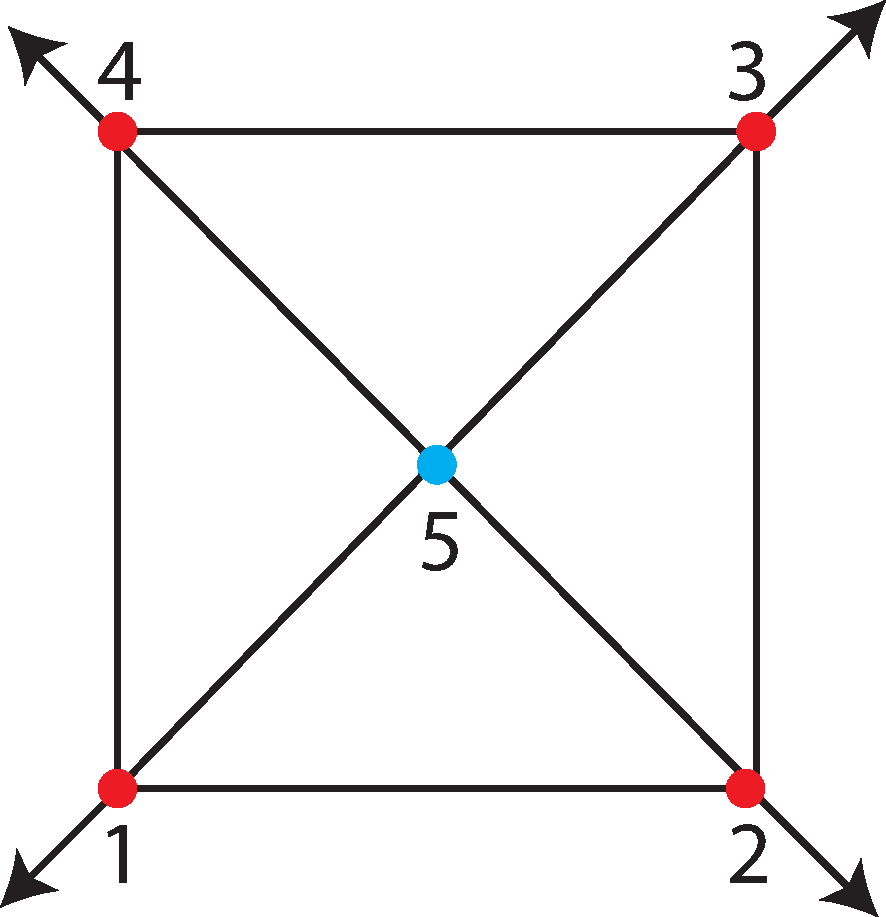
\includegraphics[width=0.8\linewidth]{images/mesh-simple.pdf}
        \caption{Malha com nós de fronteira}
    \end{figure}
    \end{columns}
\end{frame}

%------------------------------------------------

\begin{frame}
\frametitle{Solução: Nós Fantasma}
    \begin{block}{Ideia Central}
        \begin{itemize}
            \item Criar nó temporário fora do domínio
            \item Balancear estêncil de fronteira
            \item Eliminar dependência através da condição de Neumann
        \end{itemize}
    \end{block}

    \begin{figure}
        \centering
        \includegraphics[width=0.4\linewidth]{images/nring_int.png}
        \caption{Nó fantasma (ilustração conceitual)}
    \end{figure}
\end{frame}

%------------------------------------------------

\begin{frame}
\frametitle{Nós Fantasma: Formulação}
    \begin{block}{Criação do nó fantasma}
        $$\mathbf{x}_g = \mathbf{x}_b + h\mathbf{n}$$
        onde $\mathbf{n}$ é a normal à fronteira e $h = \alpha \cdot \Delta x_{local}$
    \end{block}

    \begin{block}{Condição de Neumann}
        $$\nabla p \cdot \mathbf{n} = 0 \quad \Rightarrow \quad \sum_{j}\omega_j^n p_j + \omega_g^n p_g = 0$$
    \end{block}

    \begin{block}{Eliminação do nó fantasma}
        $$p_g = -\frac{1}{\omega_g^n}\sum_{j}\omega_j^n p_j$$
    \end{block}
\end{frame}

%------------------------------------------------

\begin{frame}
\frametitle{Pesos Efetivos do Laplaciano}
    \begin{block}{Substituindo $p_g$ na aproximação do Laplaciano}
        $$\nabla^2 p \approx \sum_{j}\omega_j^L p_j + \omega_g^L p_g$$

        $$= \sum_{j}\omega_j^L p_j + \omega_g^L \left(-\frac{1}{\omega_g^n}\sum_{j}\omega_j^n p_j\right)$$

        $$= \sum_{j}\left(\omega_j^L - \frac{\omega_g^L}{\omega_g^n}\omega_j^n\right) p_j$$
    \end{block}

    \begin{block}{Pesos efetivos}
        $$\tilde{\omega}_j^L = \omega_j^L - \frac{\omega_g^L}{\omega_g^n}\omega_j^n$$
    \end{block}
\end{frame}

%------------------------------------------------

\begin{frame}
\frametitle{Interseção Raio-Polígono}
    \begin{columns}[c]
    \column{.5\textwidth}
    \begin{block}{Algoritmo}
        \begin{itemize}
            \item Cohen-Sutherland
            \item Equação paramétrica
            \item Otimização JIT (Numba)
            \item Vetorização
        \end{itemize}
    \end{block}

    \column{.5\textwidth}
    \begin{figure}
        \centering
        \includegraphics[width=\linewidth]{images/africa-nao-conforme.png}
        \caption{Exemplo de malha arbitrária}
    \end{figure}
    \end{columns}
\end{frame}

%------------------------------------------------
\section{Resultados}
%------------------------------------------------

\begin{frame}
\frametitle{Experimento 1: Validação Ghost Nodes}
    \begin{block}{Objetivo}
        Comparar método com e sem nós fantasma
    \end{block}

    \begin{itemize}
        \item Domínio: AABB simples
        \item Métrica: Divergente do campo de velocidades
        \item Resultado: Redução significativa do divergente na fronteira
    \end{itemize}
\end{frame}

%------------------------------------------------

\begin{frame}
\frametitle{Experimento 2: Geometria Irregular}
    \begin{block}{Objetivo}
        Testar capacidade em fronteiras complexas
    \end{block}

    \begin{itemize}
        \item Domínio: Polígono irregular
        \item Formação de vórtices
        \item Comportamento físico qualitativamente correto
    \end{itemize}
\end{frame}

%------------------------------------------------

\begin{frame}
\frametitle{Experimento 3: Domínio Complexo}
    \begin{block}{Objetivo}
        Validar em geometrias geográficas reais
    \end{block}

    \begin{itemize}
        \item Domínio: Contorno geográfico (país)
        \item Fronteiras altamente irregulares
        \item Demonstração de viabilidade do método
    \end{itemize}
\end{frame}

%------------------------------------------------

\begin{frame}
\frametitle{Análise do Divergente}
    \begin{block}{Observações}
        \begin{itemize}
            \item Divergente inicialmente alto (injeção de fumaça)
            \item Queda após desligamento do injetor
            \item Aumento gradual ao longo do tempo
            \item Concentração em regiões de fronteira
        \end{itemize}
    \end{block}

    \begin{block}{Interpretação}
        \begin{itemize}
            \item Ghost nodes melhoram estabilidade
            \item Desafios em regiões de alta curvatura
            \item Sensibilidade à proximidade entre nós
        \end{itemize}
    \end{block}
\end{frame}

%------------------------------------------------
\section{Discussão}
%------------------------------------------------

\begin{frame}
\frametitle{Discussão dos Resultados}
    \begin{block}{Sucessos}
        \begin{itemize}
            \item Comportamento físico qualitativamente correto
            \item Formação de estruturas vorticais
            \item Interação adequada com fronteiras
            \item Viabilidade em domínios arbitrários
        \end{itemize}
    \end{block}

    \begin{block}{Desafios Identificados}
        \begin{itemize}
            \item Perda gradual de massa
            \item Instabilidades em regiões de alta curvatura
            \item Sensibilidade à proximidade de nós
            \item Dependência da função de base radial
        \end{itemize}
    \end{block}
\end{frame}

%------------------------------------------------
\section{Conclusões e Contribuições}
%------------------------------------------------

\begin{frame}
\frametitle{Conclusões}
    \begin{block}{Principais Contribuições}
        \begin{itemize}
            \item Adaptação do Stable Fluids com RBF-FD para malhas triangulares
            \item Técnica simplificada de nós fantasma para fronteiras
            \item Algoritmo eficiente de ray-casting com JIT
            \item Demonstração de viabilidade em domínios arbitrários
        \end{itemize}
    \end{block}

    \begin{block}{Publicação}
        \begin{itemize}
            \item CNMAC 2023 - Bonito, MS
            \item "Animação de fumaça em malhas não-estruturadas usando RBF-FD"
        \end{itemize}
    \end{block}
\end{frame}

%------------------------------------------------
\section{Trabalhos Futuros}
%------------------------------------------------

\begin{frame}
\frametitle{Trabalhos Futuros}
    \begin{block}{Extensões Imediatas}
        \begin{itemize}
            \item Extensão para 3D (malhas tetraedrais)
            \item Melhoria na conservação de massa
            \item Exploração de outras funções de base radial
        \end{itemize}
    \end{block}

    \begin{block}{Desenvolvimentos Avançados}
        \begin{itemize}
            \item Domínios não-simplesmente conexos (com buracos)
            \item Otimizações de desempenho (paralelização, GPU)
            \item Refinamento adaptativo
            \item Interatividade em tempo real
        \end{itemize}
    \end{block}
\end{frame}

%------------------------------------------------

\begin{frame}
\frametitle{Agradecimentos}
\centering
    \begin{block}{}
        \begin{itemize}
            \item Prof. Dr. Afonso Paiva Neto (orientação)
            \item CAPES (bolsa PROEX)
            \item Colegas do laboratório
            \item Família e amigos
        \end{itemize}
    \end{block}

    \vspace{1cm}
    \Large{Obrigado!}

    \vspace{0.5cm}
    \normalsize{Perguntas?}
\end{frame}

%------------------------------------------------

\end{document}
